% Reconstructed from Appendix D of JobDisplacement-3.pdf (pp. 67-69), because
% its separate TeX source was not supplied. Uses the newly generated PDF assets.
In the body of the paper, the control group consists of workers who are never matched
to a displacement event over the sample period; we do not require controls to remain
continuously employed at the same firm over the post-event window. The convention
introduced by \citet{Jacobson1993}\textcolor{orange}{, which \citet{Lachowska2020} also follow,} restricts the control group to ``stayers'' continuously
employed at the same firm; \textcolor{orange}{other} recent contributions \citep{Schmieder2020,bertheau_etal_2023}
do not impose this restriction, and we follow the latter convention. As a robustness
exercise, we re-estimate the main results on the MLO30 sample using a stayer control
group, defined operationally as controls with at least six post-event years of tenure
at the matched firm. The MLO30 sample is the natural locus for this exercise: by
selecting events on a mass-layoff threshold rather than the administrative LE definition,
MLO30 is the closest mapping in our data of the construction adopted in most of the
existing literature, and is therefore the natural sample on which to assess comparability
with the JLS-style stayer convention.

Figure~\ref{fig:stayer:wages} reports the wage decomposition and Figure~\ref{fig:stayer:firms}
reports the firm-level reallocation outcomes, for both control-group definitions.
The substantive contributions of the paper---the firm wage-premium loss, the productivity
gain at destination firms, and the labor-share gap---are essentially unchanged across
the two definitions; the hours and total-earnings scars are mechanically larger under
the stayer control group, because controls subject to any subsequent separation are
excluded from the comparison pool.
\clearpage
\begin{figure}[p]
\centering
\caption{Wage decomposition on the MLO30 sample: baseline (never-displaced) vs. stayer control group}
\label{fig:stayer:wages}
\begin{subfigure}{.74\linewidth}
\caption{Baseline MLO30: never-displaced controls}
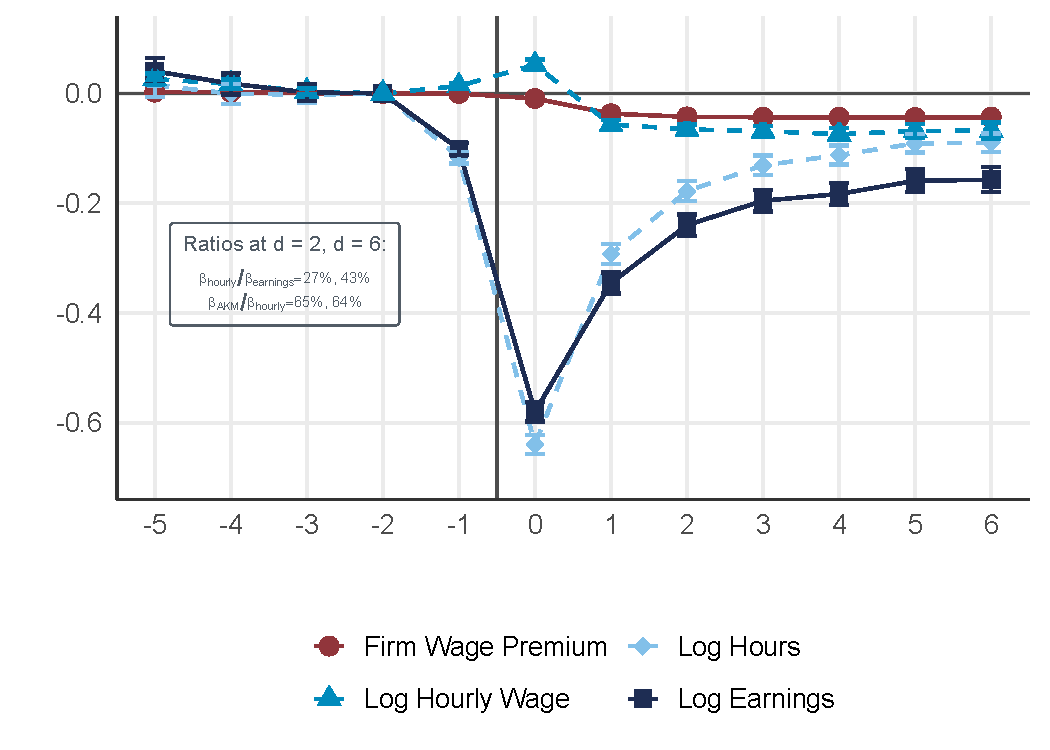
\includegraphics[width=\linewidth,max width=\linewidth]{figures/01_event_figures/figure_A18_a_mlo_baseline_wage_decomposition.pdf}
\end{subfigure}
\par\medskip
\begin{subfigure}{.74\linewidth}
\caption{Stayer MLO30: controls with at least six post-event years of tenure at the matched firm}
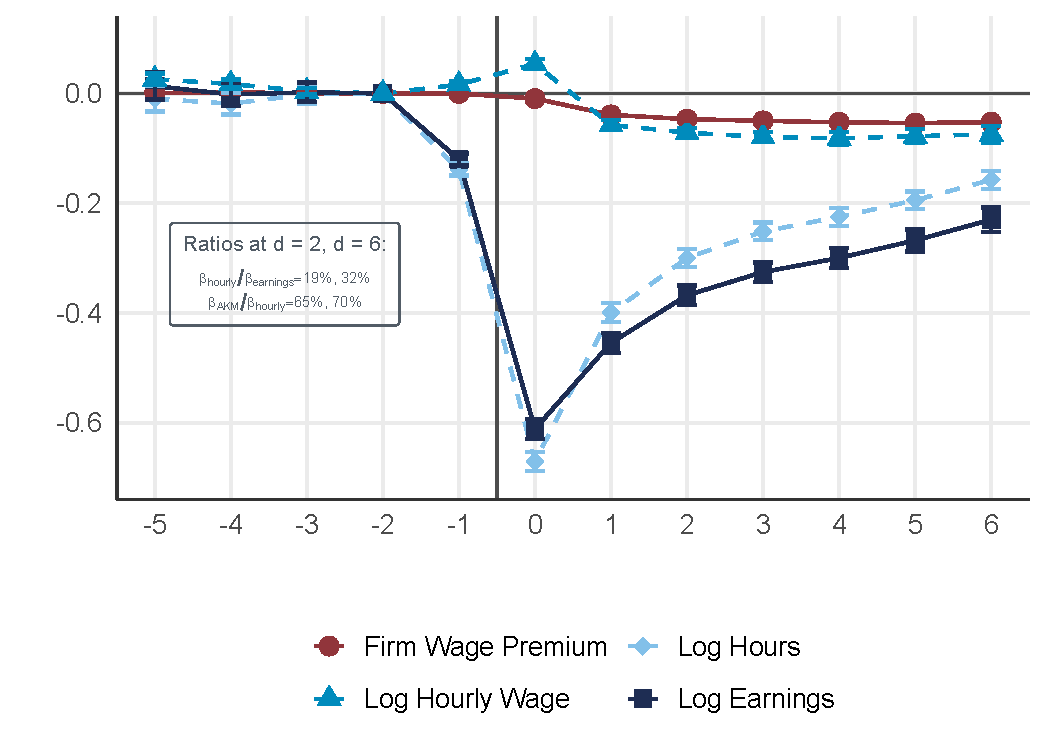
\includegraphics[width=\linewidth,max width=\linewidth]{figures/01_event_figures/figure_A18_b_mlo_stayer_wage_decomposition.pdf}
\end{subfigure}
\floatfoot{\footnotesize\textsc{Notes}: Wage decomposition for the MLO30 sample under two alternative definitions of the control group. Panel (a) uses the baseline never-displaced controls. Panel (b) uses the stayer convention of \citet{Jacobson1993}: controls continuously employed at the same firm over the post-event window. The hourly-wage scar and the firm-wage-premium loss are essentially unchanged across the two definitions; the hours and total-earnings scars are mechanically larger under the stayer convention. Standard errors: robust standard errors clustered at the worker level; displayed confidence intervals at the 99\% level.}
\end{figure}
\clearpage
\begin{figure}[p]
\centering
\caption{Productivity, labor share and firm wage premium of current employers on the MLO30 sample: baseline vs. stayer control group}
\label{fig:stayer:firms}
\begin{subfigure}{\linewidth}
\caption{Baseline MLO30: never-displaced controls}
\begin{tabular}{ccc}
Productivity & Labor share & Firm wage premium\\
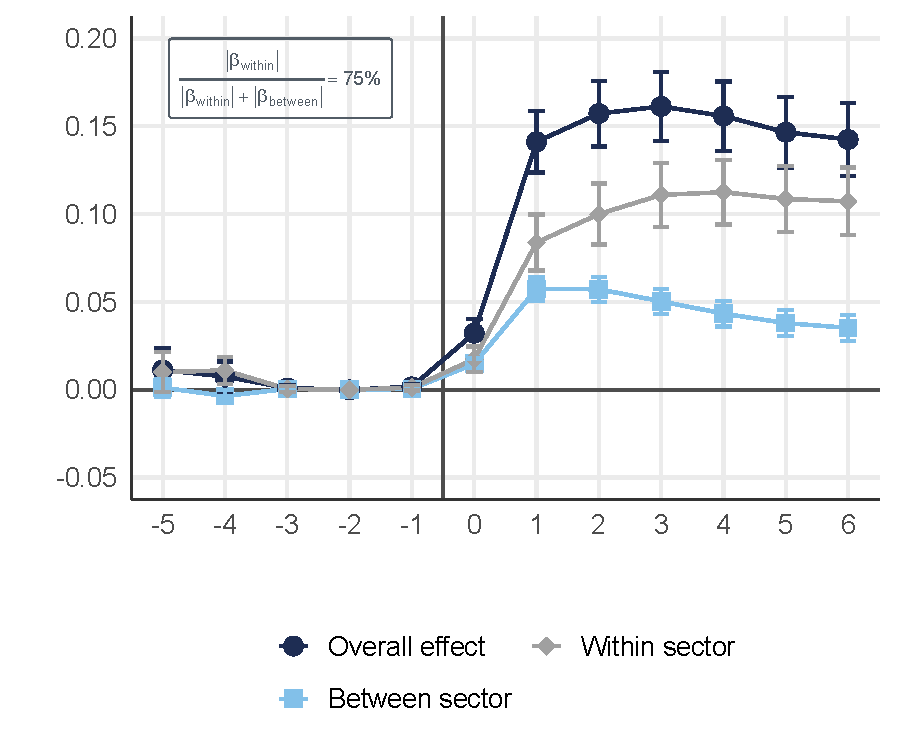
\includegraphics[width=.30\linewidth,max width=\linewidth]{figures/01_event_figures/figure_A19_a_baseline_productivity.pdf}&
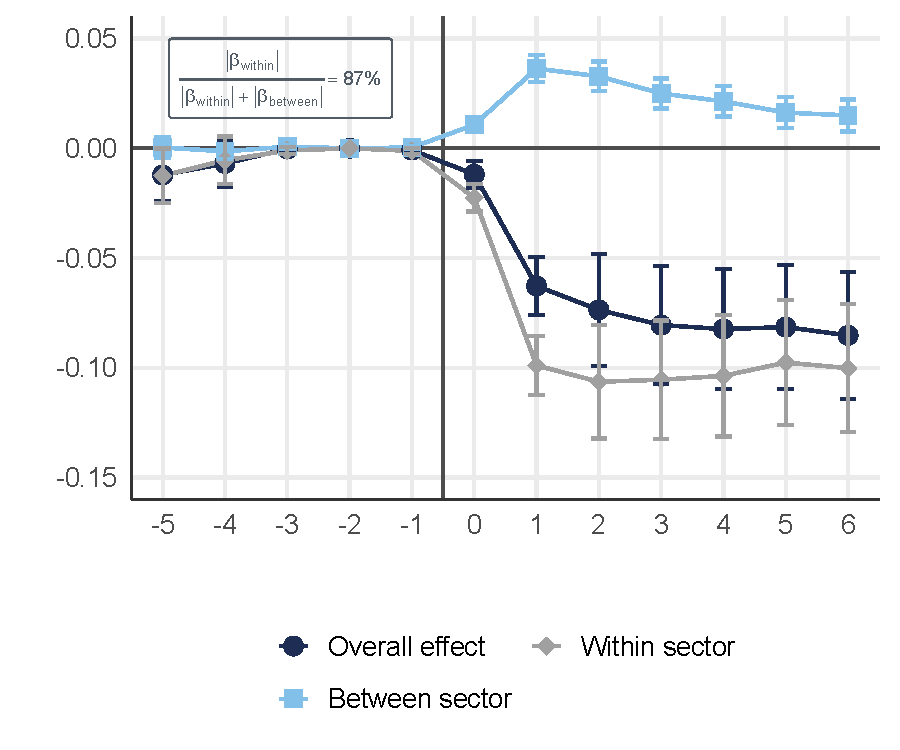
\includegraphics[width=.30\linewidth,max width=\linewidth]{figures/01_event_figures/figure_A19_a_baseline_labor_share.pdf}&
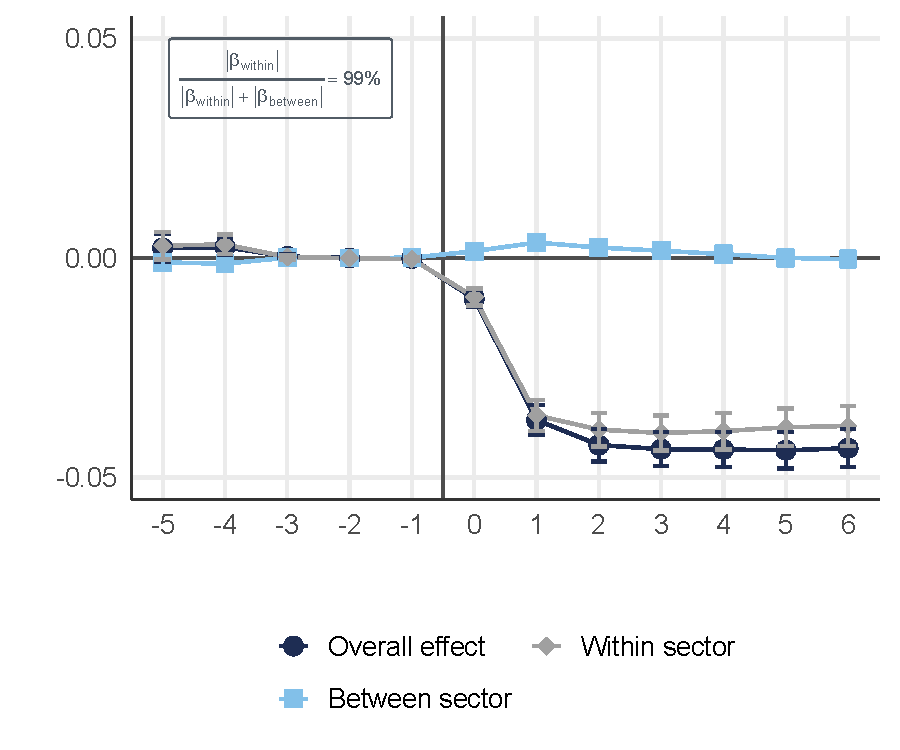
\includegraphics[width=.30\linewidth,max width=\linewidth]{figures/01_event_figures/figure_A19_a_baseline_firm_premium.pdf}
\end{tabular}
\end{subfigure}
\par\medskip
\begin{subfigure}{\linewidth}
\caption{Stayer MLO30: controls with at least six post-event years of tenure at the matched firm}
\begin{tabular}{ccc}
Productivity & Labor share & Firm wage premium\\
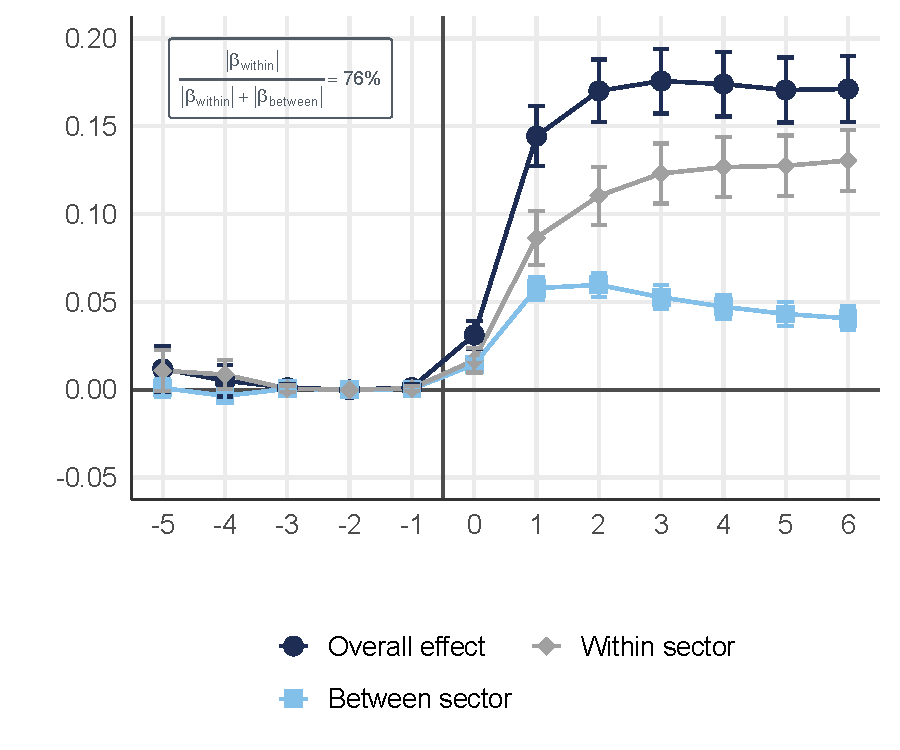
\includegraphics[width=.30\linewidth,max width=\linewidth]{figures/01_event_figures/figure_A19_b_stayer_productivity.pdf}&
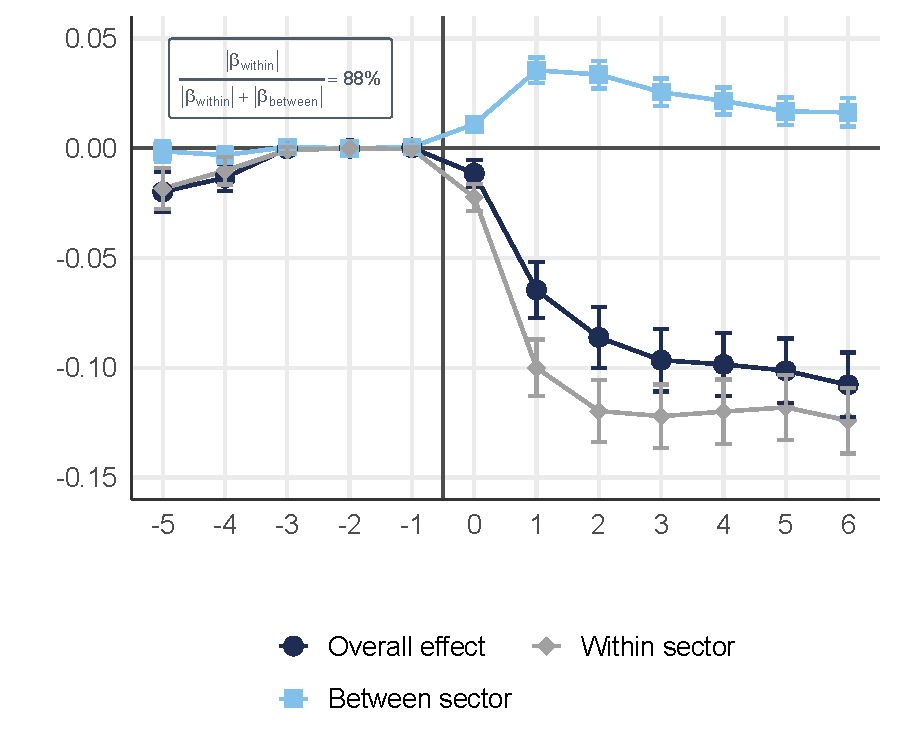
\includegraphics[width=.30\linewidth,max width=\linewidth]{figures/01_event_figures/figure_A19_b_stayer_labor_share.pdf}&
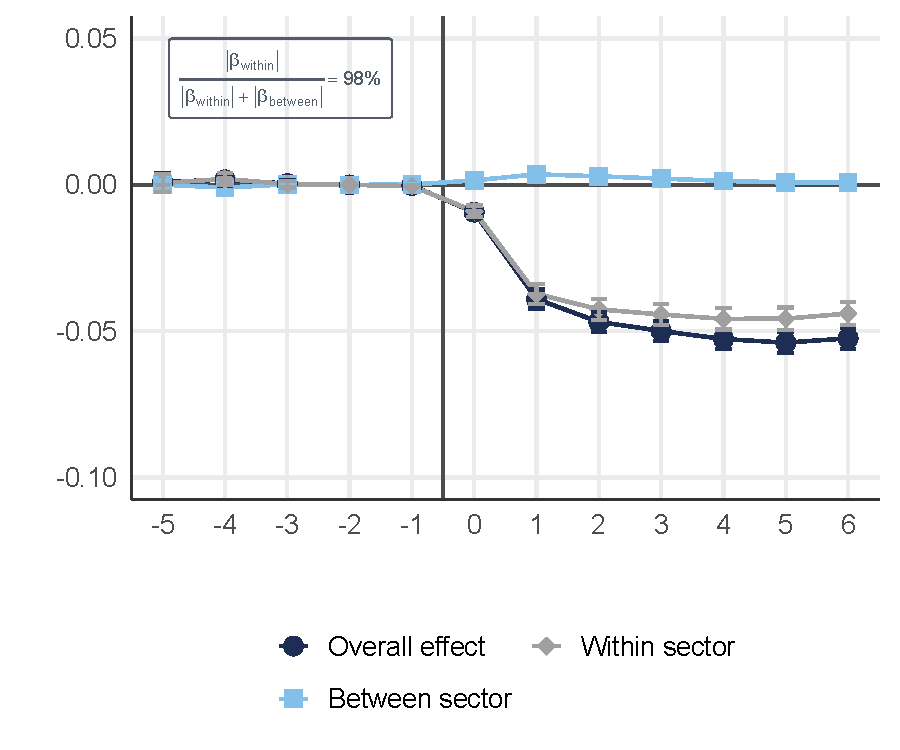
\includegraphics[width=.30\linewidth,max width=\linewidth]{figures/01_event_figures/figure_A19_b_stayer_firm_premium.pdf}
\end{tabular}
\end{subfigure}
\floatfoot{\footnotesize\textsc{Notes}: Firm-level reallocation outcomes (productivity, labor share, AKM firm wage premium of current employers) for the MLO30 sample under two alternative definitions of the control group. Panel (a) uses the baseline never-displaced controls. Panel (b) uses the stayer convention of \citet{Jacobson1993}. Standard errors: robust standard errors clustered at the worker level; displayed confidence intervals at the 99\% level.}
\end{figure}
\clearpage
